\documentclass[english]{sbrt}
\usepackage[english]{babel}
\usepackage[utf8]{inputenc}
\usepackage[acronym]{glossaries}

\newtheorem{theorem}{Theorem}

\usepackage{booktabs}
\usepackage{multirow}
\usepackage{array}
\usepackage{graphicx}
\usepackage{subcaption}
\usepackage{amsfonts}
\usepackage{xcolor}
\usepackage{tikz}
\usepackage{algorithm}
\usepackage{algpseudocode}
\usepackage{flushend}
%% ---------------------------------------------

\begin{document}

\newacronym{sbrt}{SBrT}{Brazilian Telecommunication Society}
\newacronym{sbrt2026}{SBrT~2026}{XLIV Brazilian Symposium on Telecommunication and Signal Processing}
\newacronym{ufba}{UFBA}{Federal University of Bahia}

\newacronym{ibge}{IBGE}{Brazilian Institute of Geography and Statistics}
\newacronym{anatel}{ANATEL}{Brazilian National Telecommunications Agency}
\newacronym{iqs}{IQS}{Service Quality Index}
\newacronym{rqual}{RQUAL}{Regulation on the Quality of Telecommunications Services}
\newacronym{dvr}{DVR}{Reference Values Document}
\newacronym{qos}{QoS}{Quality of Service}
\newacronym{qoe}{QoE}{Quality of Experience}
\newacronym{knn}{$k$NN}{$k$-Nearest Neighbors}
\newacronym{gnn}{GNN}{Graph Neural Networks}
\newacronym{pca}{PCA}{Principal Component Analysis}


\renewcommand{\algorithmicrequire}{\textbf{Input:}}

\newcommand{\iqsrev}{\mathrm{QoS}_\mathrm{rev}}
\newcommand{\iqsleg}{\mathrm{QoS}_\mathrm{leg}}
% TODO: adicionar uma nota de rodapé falando que o QoS_{x} é o IQS

\newcommand{\Xraw}{\mathbf{X}}
\newcommand{\xraw}{\mathbf{x}}

\newcommand{\Xpareto}{\mathbf{X}^{\mathcal{P}}}
\newcommand{\xpareto}{\mathbf{x}^{\mathcal{P}}}

\newcommand{\Xmodel}{\tilde{\mathbf{X}}}
\newcommand{\xmodel}{\tilde{\mathbf{x}}}

\newcommand{\Xlog}{\mathbf{X}^\mathrm{log}}
\newcommand{\xlog}{\mathbf{x}^\mathrm{log}}

\title{A GNN-Based Framework for Multi-Objective Telecommunications Quality Ranking}

\author{Gabriel Luiz Espindola Pedro, Paulo Ricardo Branco da Silva, Dimas Irion
    Alves, João Vitor Rosa  Negri, \\ Arthur Cadore Matuella Barcella, Renato
    Machado, Kai de Andrade Lima, and Paulo Roberto Silva Marcos \thanks{Gabriel
        Luiz Espindola Pedro, Paulo Ricardo Branco da Silva, Arthur Cadore Matuella
        Barcella, João Vitor Rosa Negri, and Dimas Irion Alves are with
        Telecommunications Department of Aeronautics Institute of Technology, São
        José dos Campos, SP, Brazil, e-mails: \{gabrielluizep, dimasirion, negri,
        pbranco, arthurcadore, rmachado\}@ita.br; Kai de Andrade Lima and Paulo
        Roberto Silva Marcos are with Agência Nacional de Telecomunicações (ANATEL),
        Brasília, Distrito Federal; e-mails: \{kai.lima, paulorsm\}@anatel.gov.br.
        This study was financed in part by the Coordenação de Aperfeiçoamento de
        Pessoal de Nível Superior - Brasil (CAPES) - Finance Code  001, Anatel under
        Decentralized Execution Agreement (TED) No. 03/2023, Work Program:
        24.722.2205.20ZD.0001, and São Paulo Research Foundation (FAPESP) under
        grant 2020/09838-0 (BIOS---Brazilian Institute of Data Science).}%
}

\maketitle

\markboth{XLIV BRAZILIAN SYMPOSIUM ON TELECOMMUNICATIONS AND SIGNAL PROCESSING - SBrT 2026, SEPTEMBER 29--OCTOBER 02, 2026, SALVADOR, BA}{}


\begin{abstract}
    Assessing telecommunications mobile services quality across municipalities
    with heterogeneous structural, geographic, and socioeconomic conditions
    requires methodologies beyond simple scalar or functional aggregations. This
    paper introduces a self-supervised Graph Neural Network (GNN) based ranking
    framework that learns the geometry of municipality-level Quality of Service
    (QoS) indicators on a $k$-nearest-neighbor graph, producing a unified
    ranking obtained by self-supervised learning on Pareto-inspired proxies. The
    architecture employs residual graph convolutional layers and is trained with
    a multi-objective loss function that enforces pairwise ranking consistency,
    input reconstruction fidelity, geometric smoothness on the learned manifold,
    and directional alignment with a Pareto-inspired proxy. The approach is
    validated on a dataset covering Brazilian municipalities over multiple
    monthly periods, totaling over 82,000 municipality--month observations.
    Results show that the proposed model produces scores with a wider effective
    range ($\sigma=0.098$) than ANATEL's legacy QoS ($\sigma=0.054$) and its
    revised version ($\sigma=0.058$) baselines, improving rank discrimination.
    Distribution and spatial analyses suggest that the framework produces more
    informative and distinguishable municipality rankings than the baselines,
    mitigating the concentration effects observed in current regulatory
    composite indicators.
\end{abstract}

\begin{keywords}
    Learn to Rank, Graph Neural Networks, Pareto Dominance, Multi-Objective
    Optimization, Quality of Service
\end{keywords}

\section{Introduction}

International best practices advocate results-based regulatory approaches for
\gls{qos}. Given the multidimensional nature of \gls{qos} indicators,
municipality ranking provides support in the prioritization of regulatory
actions. Recent works have explored data-driven approaches for ranking that go
beyond traditional aggregation, including graph-neural-network-based \gls{qos}
prediction~\cite{liu2024qosgnn,wang2025trust}, deep-learning-based \gls{qoe}
assessment for wireless networks~\cite{zhang2024assessing}, and modern Learning
to Rank techniques that learn scoring functions directly from
data~\cite{li2026s3prank}.

Defining a suitable ranking strategy is not trivial. The multidimensional nature
of telecommunications quality---encompassing network and customer-related
aspects---means that different indicators can lead to conflicting orderings, a
characteristic of multi-objective optimization
problems~\cite{suresh2024machine,kesireddy2024elite}. Establishing a definitive
ground-truth ranking is difficult; evaluating model outputs relies on
partial-ordering frameworks and domain-specific contextual knowledge. Selecting
the essential variables for ranking definition is equally unclear: not only
\gls{qos} indicators are required, but also covariates such as infrastructure
and \gls{qoe} indicators.

In multi-objective settings, Pareto dominance provides a natural partial
ordering: municipality $A$ dominates municipality $B$ if $A$ is at least as good
in every dimension and strictly better in at least
one~\cite{haxhiraj2025pareto}. However, many municipality pairs are not
comparable under strict Pareto ordering, motivating the search for a principled
scalarization rule that extends this partial order into a total order while
still respecting the dominance structure of the data. The core challenge is
therefore not only aggregation, but learning a scoring function that faithfully
accounts for each attribute's contribution---so that entities which differ in
even one dimension are consistently and meaningfully separated in the induced
ranking.

\gls{anatel} consolidates \gls{qos} indicators at the municipal level through
the \gls{iqs}, a linear composite based on weighted aggregation for each
provider and semester~\cite{anatel2025ri444,anatel2021ri71}. This approach
aligns with international practices and reflects a broader trend of deriving
orderings from multidimensional \gls{qos} metrics via linear aggregation.
However, such non-relational formulations may fail to capture the global
structure of relative municipal performance. By ignoring dominance
relationships, scores become less discriminative, with similar entities assigned
near-identical values. As detailed in Section~\ref{sec:results}, the legacy IQS
concentrates 50\% of observations between 0.835 and 0.863, an interquartile
range of only 0.028.

To address these challenges, we propose a \gls{gnn}-based Pareto-inspired model
that learns, through pairwise competition between entities, a scalar quality
score $\hat{r}_i$ for each municipality $i$. A \gls{knn} graph over the feature
space provides the relational structure for this learning process. Experimental
results indicate that the proposed multi-objective scheme expands score
dispersion and improves rank discriminability, yielding a more favorable
optimization manifold than unidimensional scalar approaches.

The remainder of the paper is organized as follows. Section~\ref{sec:dataset}
describes the dataset of municipality-level \gls{qos}, \gls{qoe}, and
infrastructure indicators provided by \gls{anatel}, along with the two
regulatory composites used as baselines. Section~\ref{sec:methodology} details
the preprocessing pipeline, graph construction, model architecture, and the
multi-objective loss function that jointly drives the ranking optimization.
Section~\ref{sec:results} evaluates the proposed model against the regulatory
baselines through distribution and geographic analyses.
Section~\ref{sec:conclusions} summarizes the main findings and outlines
directions for future work.

\section{Dataset and Baseline Creation} \label{sec:dataset}

The dataset comprises mobile service \gls{qos} and \gls{qoe} indicators and
infrastructure covariates provided by \gls{anatel}, creating a matrix $\Xraw \in
    \mathbb{R}^{N \times D}$, where $N$ corresponds to the number of
municipality--period entities and $D$ corresponds to the number of features. The
matrix $\Xraw$ is indexed by two keys: \textit{month}, which identifies the
observation period, and a unique \textit{municipality identifier}. Each row,
therefore, corresponds to one municipality--month pair. Since not all selected
features are available at monthly granularity, interpolation schemes are applied
where necessary.

The eight indicators available related to mobile service are selected and
normalized to $[0,1]$: $\mathrm{IND}_1$ (voice-call connection rate),
$\mathrm{IND}_2$ (voice-call drop rate), $\mathrm{IND}_3$ (data-connection
rate), $\mathrm{IND}_4$ (download and upload speed compliance rate),
$\mathrm{IND}_5$ (data-connection latency), $\mathrm{IND}_6$ (jitter),
$\mathrm{IND}_7$ (packet-loss rate), and $\mathrm{IND}_8$ (service availability
rate). In addition, $\mathrm{INF4}_{\mathrm{UP},\{\mathrm{3G,4G,5G}\}}$ and
$\mathrm{INF4}_{\mathrm{DL},\{\mathrm{3G,4G,5G}\}}$ indicators are provided,
which record the median upload and download speeds over each mobile data
technology, respectively. For \gls{qoe}, the $\mathrm{ISG}$ (General
Satisfaction Index) was selected as a composite of \gls{qoe} indicators for a
given municipality--period tuple. Infrastructure is represented by the
$\mathrm{IBC}$ (Brazilian Coverage Index).

To establish a baseline comparison, we adopt the two \gls{iqs} composite
scores\footnote{The \gls{iqs} (Índice de Qualidade do Serviço) is referred to by
    \gls{anatel} as the official \gls{qos} composite indicator.}. The \gls{iqs} is
officially published on a semi-annual basis, indexed by provider and
municipality, with the primary objective of monitoring and evaluating
telecommunications service quality in Brazil through a transparent and
comparative indicator of provider
performance~\cite{anatel2025ri444,anatel2021ri71}.

For our analysis, we derive monthly estimates aggregated at the municipality
level by averaging across providers. The legacy composite $\iqsleg =
    \sum_{k=1}^{K} w_k^{\mathrm{leg}}\,\mathrm{IND}_k$, in use since November 2021,
uses fixed weights $w^{\mathrm{leg}} = (0.1, 0.1, 0.1, 0.2, 0.1, 0.1, 0.1,
    0.2)$, assigning greater relevance to $\mathrm{IND}_4$ and $\mathrm{IND}_8$
\cite{anatel2021ri71}. The revised composite $\iqsrev$, replacing the legacy
since June 2025, adopts a performance-dependent scheme: indicators are ranked
from worst to best within each municipality--period and assigned the
inverse-harmonic weight $\alpha_r = 1/(r\,H_K)$, where $H_K =
    \sum_{j=1}^{K}1/j$, so that $\iqsrev = \sum_{r=1}^{K}
    \alpha_r\cdot\mathrm{IND}_{\pi(r)} + B_{\mathrm{cov}}$, with $\pi$ consisting in
a permutation that orders indicators from worst to best and $B_{\mathrm{cov}}$
consisting in a five-point bonus awarded when 4G or higher coverage reaches at
least 95\% in the urban area \cite{anatel2025ri444}.

\section{Methodology} \label{sec:methodology}

The proposed ranking framework transforms raw municipality indicators into a
scalar ranking score through pairwise dominance-guided learning on a
graph-structured representation. The pipeline comprises four stages:
preprocessing of raw indicators, detailed in Section~\ref{sec:preproc}; graph
construction in Section~\ref{sec:graph}; positional encoding in
Section~\ref{sec:pe}; and a residual graph convolutional architecture trained
with the multi-objective loss described in Section~\ref{sec:loss}.

\subsection{Preprocessing} \label{sec:preproc}

The selected features exhibit heavy-tailed distributions and marked
heterogeneity in scale and support range---characteristics observed empirically
across infrastructure and \gls{qos} indicators in the dataset.
Algorithm~\ref{alg:preprocessing} details the full preprocessing pipeline, which
takes $\Xraw$ as input and produces two output matrices: $\Xmodel$, used as
input to the model, and the Pareto dominance proxy matrix $\Xpareto$, used as a
directional target during training. The pipeline first applies a Log1p
transform, $x \mapsto \log(1+x)$, to compress heavy tails. Next, Robust Scaling
centers each feature by its median and divides by the interquantile range
$Q_{0.95} - Q_{0.05}$, which is more resilient to outliers than the full range.
Standard Scaling is then applied sequentially to yield $\Xmodel$ with zero mean
and unit variance, ensuring that no single feature dominates gradient updates.
In parallel, Min-Max scaling on $\Xlog$ produces $\Xpareto \in [0,1]^{N \times
        D}$, from which a scalar surrogate utility $u_i$ is derived as the feature-wise
mean; since all features are normalized to $[0,1]$ and oriented so that higher
values denote better performance, this average provides a consistent monotone
direction for training in the absence of labeled rankings.

\begin{algorithm}
    \caption{Preprocessing Pipeline}
    \label{alg:preprocessing}
    \begin{algorithmic}[1]
        \Require $\Xraw \in \mathbb{R}^{N \times D}$, raw indicator matrix
        \State $\Xlog \gets \log(1 + \Xraw)$
        \Comment{Log1p Transform}
        \For{each feature $j = 1, \ldots, D$}
        \State $\tilde{x}_{:,j} \gets
            \dfrac{\xlog_{:,j} - \mathrm{median}(\xlog_{:,j})}
            {Q_{0.95}(\xlog_{:,j}) - Q_{0.05}(\xlog_{:,j})}$
        \Comment{Robust Scaling}
        \EndFor
        \For{each feature $j = 1, \ldots, D$}
        \State $\Xmodel_{:,j} \gets
            \dfrac{\tilde{x}_{:,j} - \mathrm{mean}(\tilde{x}_{:,j})}
            {\mathrm{std}(\tilde{x}_{:,j})}$
        \Comment{Standard Scaling}
        \EndFor
        \For{each feature $j = 1, \ldots, D$}
        \State $\Xpareto_{:,j} \gets
            \dfrac{\xlog_{:,j} - \min_i \xlog_{i,j}}
            {\max_i \xlog_{i,j} - \min_i \xlog_{i,j}}$
        \Comment{Pareto Proxy (Min-Max on $\Xlog$)}
        \EndFor
        \For{each entity $i = 1, \ldots, N$}
        \State $u_i \gets \frac{1}{D}\sum_j \Xpareto_{i,j}$
        \EndFor
        \Ensure $\Xmodel \in \mathbb{R}^{N \times D}$ (model input),\;
        $\Xpareto \in [0,1]^{N \times D}$,\;
        $u_i \in [0,1]$ (ranking surrogate)
    \end{algorithmic}
    \vspace{-1.5em}
\end{algorithm}

\subsection{Graph Construction and Relational Structure} \label{sec:graph}

A directed \gls{knn} graph $\mathcal{G} = (\mathcal{V}, \mathcal{E})$ is
constructed over the preprocessed feature space $\Xmodel$, where $\mathcal{V}$
is the set of nodes and $\mathcal{E}$ the set of directed edges. Each
municipality--period is represented by a node $v_i \in \mathcal{V}$, and edges
encode feature-space proximity between entities.

The graph is constructed using \gls{knn} on $\Xmodel$ with a Minkowski distance
metric, yielding a neighbor matrix $\mathcal{I} \in \{1,\ldots,N\}^{N \times k}$
where each row $\mathcal{I}_{i,:}$ lists the $k$ nearest neighbors of node $i$.
The resulting graph is directed: edges $(i \rightarrow j)$ are generated for
each $j \in \mathcal{I}_{i,:}$.

\subsection{Positional Encoding} \label{sec:pe}

Message-passing GNNs possess a permutation-equivariance property: relabeling
nodes does not change the computation as long as edges and features are
relabeled consistently~\cite{dai2025survey}. While this invariance is generally
desirable, it also means the network lacks the notion of absolute coordinates
for its nodes. To inject this structural awareness, we compute positional
encodings $p_i \in \mathbb{R}^{d_{pe}}$.

We employ \gls{pca}, which finds the orthogonal directions of maximum variance
in $\Xmodel$ and projects onto the top components; each node thus receives a
low-dimensional coordinate reflecting its position in the global data
distribution.

While alternative methods---such as spectral embeddings based on the graph
Laplacian or non-linear manifold techniques---can provide richer positional
encodings, \gls{pca} is adopted here as a computationally efficient linear
approximation suitable for the dataset scale.

The computed features $p_i$ are standardized and concatenated with the original
node data $x_i$, ensuring that the positional coordinates do not dominate as a
result of disproportionate magnitudes.

\subsection{Model Architecture}

The core processing logic is built upon message-passing, generalizing the
spectral graph convolution introduced in~\cite{kipf2017semi}. At each layer
$\ell$, a node representation $h_i^{(\ell)}$ is updated by aggregating features
from its neighbors via

\begin{equation}
    m_i^{(\ell)} = \mathrm{AGG}
    \left(\left\{
    \phi\left(h_j^{(\ell)}\right):(j\rightarrow i) \in E
    \right\}\right),
\end{equation}
with each subsequent layer computed as
\begin{equation}
    h_i^{(\ell+1)} = \psi\left(h_i^{(\ell)},m_i^{(\ell)}\right),
\end{equation}

\noindent
where $\phi$ is a learnable linear transformation, $\mathrm{AGG}$ is a
permutation-invariant aggregator (mean pooling), and $\psi$ combines the
aggregated messages with the node's current state through a learnable affine
transformation followed by a non-linear activation~\cite{amara2025multiview}.

The proposed ranking framework uses Residual Graph Convolutional (ResGCN) blocks
for $\psi$, incorporating skip-connections following the original residual
learning paradigm~\cite{he2016deep,scholkemper2025residual}. Given the node
feature matrix $X \in \mathbb{R}^{n \times d_{\text{in}}}$ for a subgraph with
$n$ nodes and $d_{\text{in}}$ input features, with the edge list stored in COO
(Coordinate) format as source--target index arrays, each ResGCN layer computes

\begin{equation}
    \begin{aligned}
        H         & = X W_{\mathrm{proj}}^\top + b_{\mathrm{proj}},           \\
        \bar{H}_i & = \frac{\sum_{(j \to i) \in E} H_j}{\deg_i + \epsilon},   \\
        X^\prime  & = \mathrm{GELU}\!\left(\bar{H} + \mathrm{skip}(X)\right),
    \end{aligned}
\end{equation}

\noindent
where $W_{\mathrm{proj}}$ and $b_{\mathrm{proj}}$ are learnable weights and
bias, $\deg_i$ is the in-degree of node $i$, and $\epsilon$ is a small stability
constant. The skip path is the identity when dimensions match or a linear
projection otherwise; this residual structure shortens gradient paths, improving
trainability and mitigating oversmoothing---the convergence of node
representations under repeated neighborhood
aggregation~\cite{scholkemper2025residual,akansha2025oversquashing}.

Due to the rapid computational growth associated with neighborhood scaling,
bounded graph subsampling via breadth-first search with neighbor downsampling is
employed. At each hop, neighbor lists are randomly subsampled to a fixed limit,
and a hard cap on the total number of nodes is enforced. This enables
memory-efficient training by transferring only small induced subgraphs to the
processing device at each step, at the cost of reduced long-range message
propagation per step, which stochastic sampling across iterations mitigates.

All activations use the Gaussian Error Linear Unit (GELU), achieving smooth,
continuously differentiable non-linearity. The GELU activation function is
monotone increasing for positive and small negative values; coupled with the
model components, this property satisfies monotonicity constraints: positive
variations in individual \gls{qos} metrics consistently translate to
non-decreasing scores.

The model functions as a multi-task architecture with two output heads from the
final representations: (1) a \textit{ranking head} that maps the node embedding
to a scalar score $\hat{r}_i \in [0,1]$ via an MLP with sigmoid output; and (2)
a \textit{reconstruction head} that maps the embedding back to the original
feature space. The reconstruction head acts as an autoencoder regularizer,
discouraging degenerate solutions where ranking constraints are satisfied but
the intermediate representation discards input information. Each of these
objectives is formalized through a dedicated loss term, as described in the
following subsection.

\subsection{Training Objectives and Loss Terms} \label{sec:loss}

The model uses a weighted sum of four loss terms to jointly optimize
complementary perspectives, yielding a scalarized solution more balanced and
robust than one-dimensional optimization

\begin{equation}
    \begin{aligned}
        \mathcal{L} & =
        \lambda_\mathrm{comp} \mathcal{L}_\mathrm{comp} +
        \lambda_\mathrm{recon} \mathcal{L}_\mathrm{recon} \\
                    & +
        \lambda_\mathrm{rank} \mathcal{L}_\mathrm{rank} +
        \lambda_\mathrm{geo} \mathcal{L}_\mathrm{geo},
    \end{aligned}
\end{equation}

The Compass Loss $\mathcal{L}_\mathrm{comp}$ aligns model scores with the proxy
$u_i$, providing a monotone directional signal during training

\begin{equation}
    \mathcal{L}_{\mathrm{comp}} = \frac{1}{|B|} \sum_{i \in B} (s_i - u_i)^2.
\end{equation}

\noindent
where $i$ indexes each sample in the current mini-batch $B$.

The Reconstruction Loss $\mathcal{L}_\mathrm{recon}$ evaluates the decoder's
ability to recover the original standardized features, enforcing information
preservation

\begin{equation}
    \mathcal{L}_{\mathrm{recon}}
    = \frac{1}{|B|} \sum_{i \in B} \|\mathbf{\hat{x}}_i - \xmodel_i\|_2^2.
\end{equation}

The Pairwise Ranking Loss $\mathcal{L}_\mathrm{rank}$ establishes ordering
constraints via margin-based pairwise comparisons: the loss penalizes any pair
whose predicted score gap falls below a minimum margin $m$ relative to the
ordering induced by the proxy. This follows the classical RankNet
formulation~\cite{burges2005learning} and its neural
extensions~\cite{koppel2025pairwise}. For two entities $A$ and $B$ with target
label $y = \mathrm{sign}(u_A - u_B)$, where $u_A$ and $u_B$ are the proxy
utility values of municipalities $A$ and $B$, respectively, we have that

\begin{equation}
    \mathcal{L}_{\mathrm{rank}}
    = \frac{1}{|P|} \sum_{(A,B) \in P} \max(0, m - y(s_A - s_B)),
\end{equation}

\noindent
where the margin $m$ serves a dual purpose: it demands a minimum score
separation between pairs ordered by the proxy, and it suppresses the
contribution of pairs whose proxy difference $|u_A - u_B|$ is small---and
therefore potentially unreliable---by allowing the loss to reach zero before
perfect separation is achieved. Pairs that violate the margin constraint are
penalized linearly, while correctly ordered pairs with sufficient separation
contribute zero loss.

The Geometric Smoothness Loss $\mathcal{L}_\mathrm{geo}$ encourages score
consistency among neighboring nodes by penalizing large score differences across
edges, following the discrete Dirichlet energy---the sum of squared signal
differences along all edges---on the graph

\begin{equation}
    \label{eq:l_geo}
    \mathcal{L}_{\mathrm{geo}}
    =  \frac{1}{|E_{\mathrm{sub}}|}
    \sum_{(i,j) \in E_{\mathrm{sub}}} (s_i - s_j)^2,
\end{equation}

\noindent
where $E_{\mathrm{sub}}$ is the edge set of the current subgraph sample. Since
graph edges connect municipalities that are similar in feature space, this term
enforces that nearby entities receive comparable scores. A conservative weight
prevents oversmoothing, preserving meaningful score variation across the
distribution.

\section{Results and Discussion} \label{sec:results}

We evaluate the proposed ranking framework against the regulatory baselines
using distribution and geographic analyses across 82{,}462 municipality--period
observations. The legacy composite $\iqsleg$ concentrates scores in a narrow
band ($\sigma = 0.054$, \gls{iqr} $= 0.028$), and the revised $\iqsrev$ offers
only marginal improvement ($\sigma = 0.058$, \gls{iqr} $= 0.028$). In contrast,
the proposed score $\hat{r}$ achieves $\sigma = 0.098$ and \gls{iqr} $=
    0.137$---a 1.8 times and nearly five times expansion relative to $\iqsleg$,
respectively---enabling finer municipality rank differentiation with distinct
performance profiles.

Fig.~\ref{fig:hist} presents overlaid histograms of the three scoring
approaches, enabling direct visual comparison of how each method distributes
municipality scores. The $\iqsleg$ distribution is comparatively more clustered:
its mass is almost entirely concentrated between $0.83$ and $0.87$, forming a
sharp, narrow peak that reflects the inability of the legacy composite to spread
municipalities across the score domain. The $\iqsrev$ distribution is slightly
wider but displays a pronounced asymmetry, with a tall peak near $0.59$ and a
long left tail extending toward $0.05$. In contrast, the proposed model's
histogram is visibly broader and flatter, with frequencies distributed more
uniformly across the range from approximately $0.22$ to $0.80$. This shape
indicates that the multi-objective optimization yields a scoring function that
more effectively utilizes the support domain, producing a more differentiated
range of performance levels.

As external validation, the proposed score achieves a Pearson correlation of
$\rho = 0.40$ with the \gls{mhdi}---independent of the intra-set
features---exceeding the baselines by $0.07$ and $0.05$, indicating that the
model captures socioeconomic structure not encoded in the linear composites.

\begin{figure}[t]
    \centering
    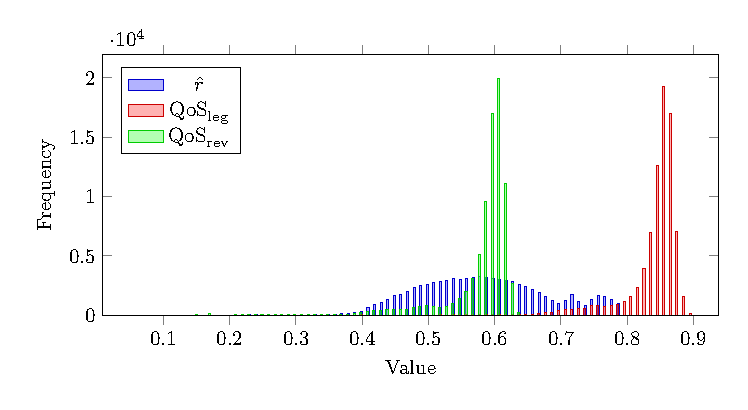
\includegraphics[width=1\linewidth]{figures/hist.pdf}
    \caption{Comparison between score and baseline distributions.}
    \label{fig:hist}
    \vspace{-1.5em}
\end{figure}

To spatially validate the framework, we selected December 2022 for evaluation,
as it corresponds to the period with the fewest missing values across
municipalities. Fig.~\ref{fig:mps} shows the comparative geographic mapping for
each metric across Brazilian municipalities. While the proposed model score
exhibits continuous performance transitions that highlight distinct geographic
regions---consistent with the distributional patterns observed in the histogram
analysis---the regulatory indicators collapse the vast majority of
municipalities into either the highest score band or a narrow intermediate
range.

The geographic contrast is particularly evident when comparing macro-regions. In
the $\iqsleg$ map, municipalities with substantially different performance
profiles are assigned nearly identical composite values, creating plateaus that
flatten the distribution---masking known infrastructure and socioeconomic
disparities between these regions. According to the \gls{mhdi} compiled by the
United Nations Development Programme, all states in the North and Northeast
present \gls{mhdi} values below the national average, in stark contrast to the
South and Southeast, where the majority of municipalities fall within the higher
development tiers~\cite{undp2023mhdi}. The $\iqsrev$ map, despite its
inverse-harmonic weighting scheme, still exhibits limited score dispersion, with
most of the territory concentrated in a narrow range---even though broad
regional contrasts, such as the separation between the North and the remaining
regions, remain discernible. The proposed framework amplifies this variation,
extending discriminability across the full score range.

The proposed model's score map reveals a clear North--South gradient consistent
with the known human development landscape across Brazilian
macro-regions~\cite{undp2023mhdi}. Municipalities in the South, Southeast, and
parts of the Center-West display higher scores, forming distinguishable
clusters. In comparison, the North and parts of the Northeast exhibit lower
scores aligned with their lower \gls{mhdi} scores~\cite{undp2023mhdi}. Even
within macro-regions, the model captures intra-regional heterogeneity: isolated
high-performing municipalities (typically state capitals or large urban centers)
are clearly visible against their surrounding rural areas, a distinction that
the baselines' compressed ranges cannot render.

\begin{figure}[t]
    \centering
    \begin{subfigure}[b]{0.24\textwidth}
        \centering
        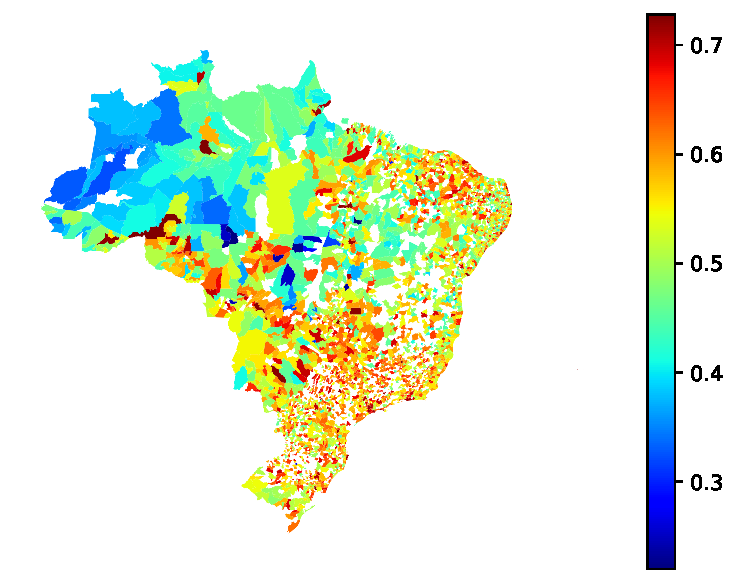
\includegraphics[width=\textwidth]{figures/map_score.pdf}
        \caption{$\hat{r}$}
        \label{fig:map_s}
    \end{subfigure}
    \hfill
    \begin{subfigure}[b]{0.24\textwidth}
        \centering
        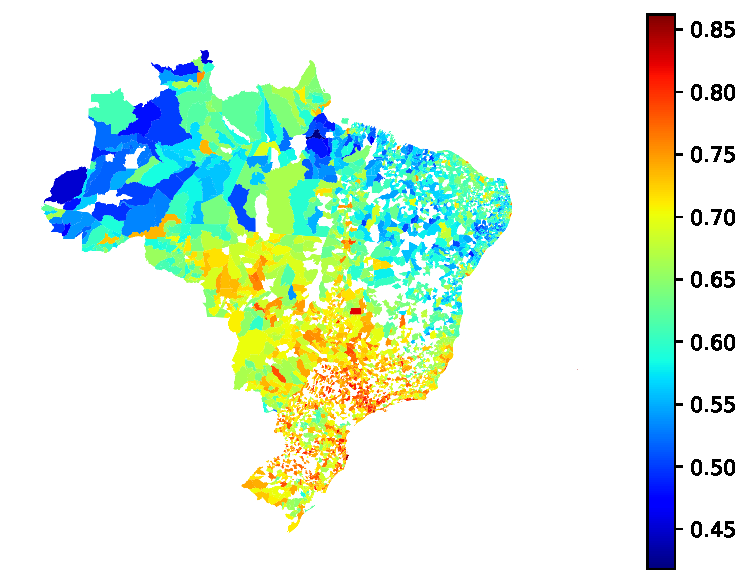
\includegraphics[width=\textwidth]{figures/map_idhm.pdf}
        \caption{MHDI}
        \label{fig:map_mdhi}
    \end{subfigure}
    \vfill
    \begin{subfigure}[b]{0.24\textwidth}
        \centering
        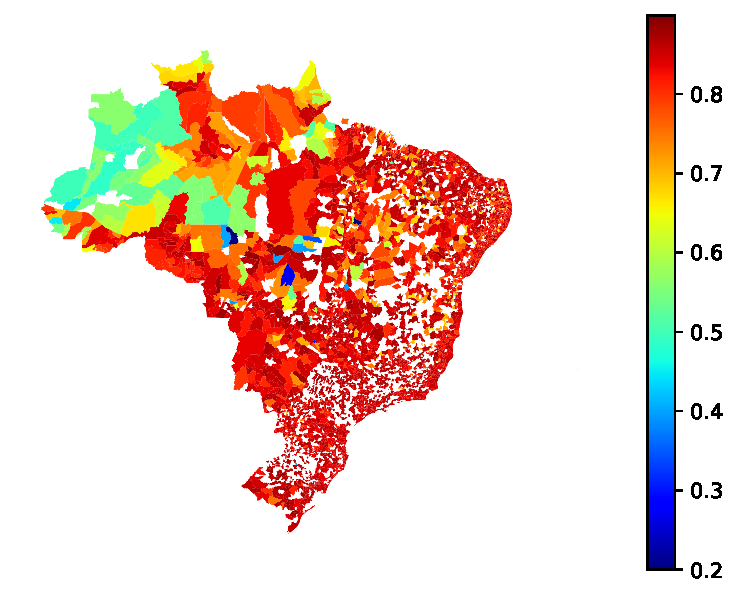
\includegraphics[width=\textwidth]{figures/map_iqs_leg_div.pdf}
        \caption{$\iqsleg$}
        \label{fig:map_iqs_leg}
    \end{subfigure}
    \hfill
    \begin{subfigure}[b]{0.24\textwidth}
        \centering
        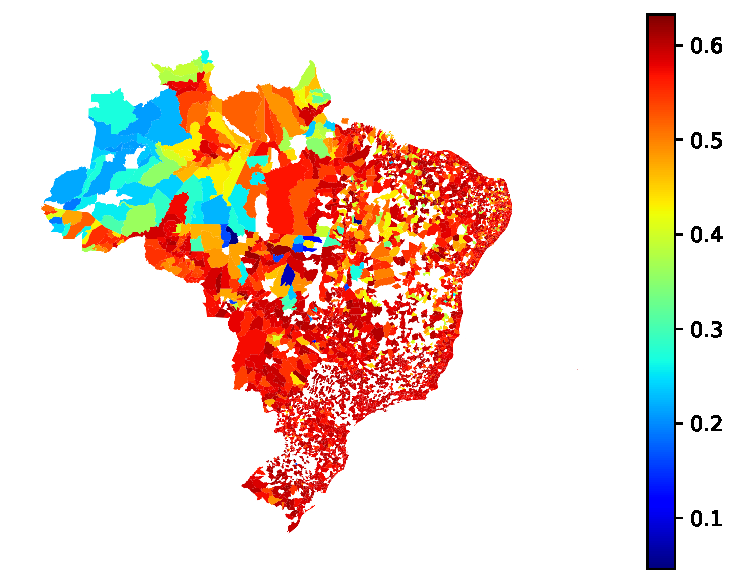
\includegraphics[width=\textwidth]{figures/map_iqs_rev_div.pdf}
        \caption{$\iqsrev$}
        \label{fig:map_iqs_ev}
    \end{subfigure}

    \caption{Geographic distribution of analysed variables for December 2022.}
    \label{fig:mps}
    \vspace{-1.5em}
\end{figure}

\section{Conclusion} \label{sec:conclusions}

While the analyzed \gls{anatel} composite indices exhibit score clustering that
limits spatial discrimination, this paper introduces a self-supervised,
Pareto-guided ranking framework that significantly expands score
discriminability across the distribution of municipalities, surpassing legacy
and revised baselines through joint optimization of competing quality
objectives.

By combining pairwise ranking, feature reconstruction, geometric smoothness, and
a directional penalty, the model's optimization covers distinct, complementary
dimensions, yielding a more balanced solution than that provided by
one-dimensional scalar optimization. The quantitative analysis demonstrates that
the proposed score achieves an interquartile range of $0.137$, representing a
nearly five times expansion compared to both baselines---\gls{iqr} $= 0.028$ for
$\iqsleg$ and \gls{iqr} $= 0.028$ for $\iqsrev$---and a standard deviation $1.8$
times larger than the $\iqsleg$. External validation against the \gls{mhdi}
shows that the proposed score correlates with \gls{mhdi} at $\rho = 0.40$,
exceeding the correlation achieved by the legacy and revised baselines by $0.07$
and $0.05$, respectively, indicating that the learned ranking captures
socioeconomic structure beyond what the linear composites encode.

Future work can benchmark the proposed approach against established
learning-to-rank methods. Strengthening the external validation with additional
covariates outside the current dataset and seemingly independent of
telecommunications metrics is also a possible direction of research. Finally,
exploring alternative positional encoding methods, such as Spectral Embedding
for non-linear manifold coordinates, and testing other activation functions to
assess infrastructural stability are also possibilities.

% \section*{Acknowledgments}

\bibliographystyle{IEEEtran}
\bibliography{references}

\end{document}
